\section{Aufbau}
\label{sec:Aufbau}

Der Versuchsaufbau besteht aus einem Ultraschallechoskop, zwei Ultraschallsonden die mit $\SI{2}{\mega\hertz}$, beziehungsweise $\SI{4}{\mega\hertz}$ betrieben werden und einem Computer zu Aufnahme und Analyse der Messdaten. Als Probe dient ein Acrylblock mit Bohrungen, die als Fehlstellen dienen (vergleiche Abbildung \ref{fig:Probe}). Als Kopplungsmittel wird destilliertes Wasser benutzt. Am Ultraschallechoskop wird die Messmethode auf Impuls-Echo-Verfahren gestellt. Zur Auswertung der Messdaten am Computer wird die Software A-Scan verwendet. Für den letzten Versuchsteil wird ein Herzmodell verwendet. Dieses besteht aus einem Doppelgefäß mit einer beweglichen Membran, die periodisch mithilfe eines Gummiballs gewölbt werden kann. 
\begin{figure}
\centering
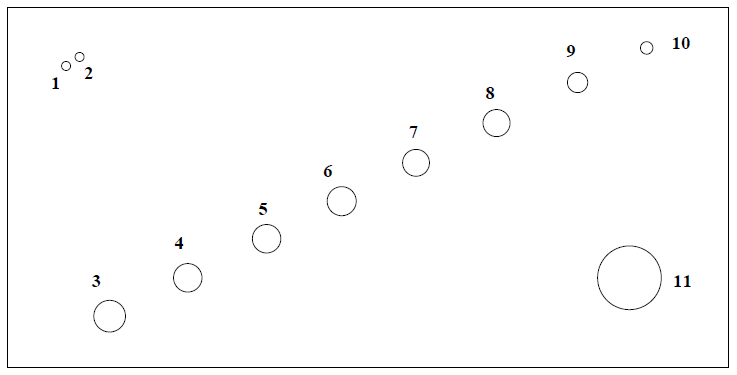
\includegraphics[scale=0.4]{content/images/Acrylblock.jpg}
\caption{Schematische Skizze des Acrylblocks \cite{US2}}
\label{fig:Probe}
\end{figure}